\documentclass[12pt,a4paper]{article}
\usepackage[utf8]{inputenc}

\usepackage{mathtools}
\usepackage{amsmath}
\usepackage{amssymb}
\usepackage{amsthm}
\usepackage{amssymb}
\usepackage{mathdots}
\usepackage[pdftex]{graphicx}
\usepackage{fancyhdr}
\usepackage[margin=1in]{geometry}
\usepackage{multicol}
\usepackage{bm}
\usepackage{listings}
\usepackage{xcolor}
\usepackage{pdfpages}
\usepackage{algpseudocode}
\usepackage{tikz}
\usepackage{enumitem}
\usepackage[T1]{fontenc}
\usepackage{inconsolata}
\usepackage{framed}
\usepackage{wasysym}
\usepackage[thinlines]{easytable}
\usepackage{hyperref}
\usepackage{minted}
\usemintedstyle{perldoc}
\hypersetup{
    colorlinks=true,
    linkcolor=blue,
    filecolor=magenta,      
    urlcolor=blue,
}
\definecolor{codegreen}{rgb}{0,0.6,0}
\definecolor{codegray}{rgb}{0.5,0.5,0.5}
\definecolor{codepurple}{rgb}{0.58,0,0.82}
\definecolor{backcolour}{rgb}{0.95,0.95,0.92}
\lstdefinestyle{mystyle}{
    backgroundcolor=\color{backcolour},   
    commentstyle=\color{codegreen},
    keywordstyle=\color{magenta},
    numberstyle=\tiny\color{codegray},
    stringstyle=\color{codepurple},
    basicstyle=\ttfamily,
    breakatwhitespace=false,         
    breaklines=true,                 
    captionpos=b,                    
    keepspaces=true,                 
    numbers=left,                    
    numbersep=5pt,                  
    showspaces=false,                
    showstringspaces=false,
    showtabs=false,                  
    tabsize=4
}
\lstset{style=mystyle}
\newcommand\numberthis{\addtocounter{equation}{1}\tag{\theequation}}
\newcommand{\rightqed}{
\begin{flushright}
$\blacksquare$
\end{flushright}
}
\newcommand{\solution}{\noindent\textbf{Solution:}\\}
\usepackage{graphics}
\usepackage{subfig}
\graphicspath{ {./images/} }

\title{CSCI 6690 Spectral Graph Theory Homework 5\\Graph coloring and spectral theory}
\author{Kushajveer Singh}
\date{}

\begin{document}
\maketitle

% Start problem 1
\subsection*{Problem 1(1)}
\textit{
    Establish upper bound on $\chi(G)$
}

\solution
Figure \ref{fig:q_1} shows a coloring of the graph $G$ with 3 colors. Based on this $\chi(G)$ is bounded as follows
\begin{equation}
    \chi(G) \leq 3
\end{equation}
\begin{figure}[H]
    \centering
    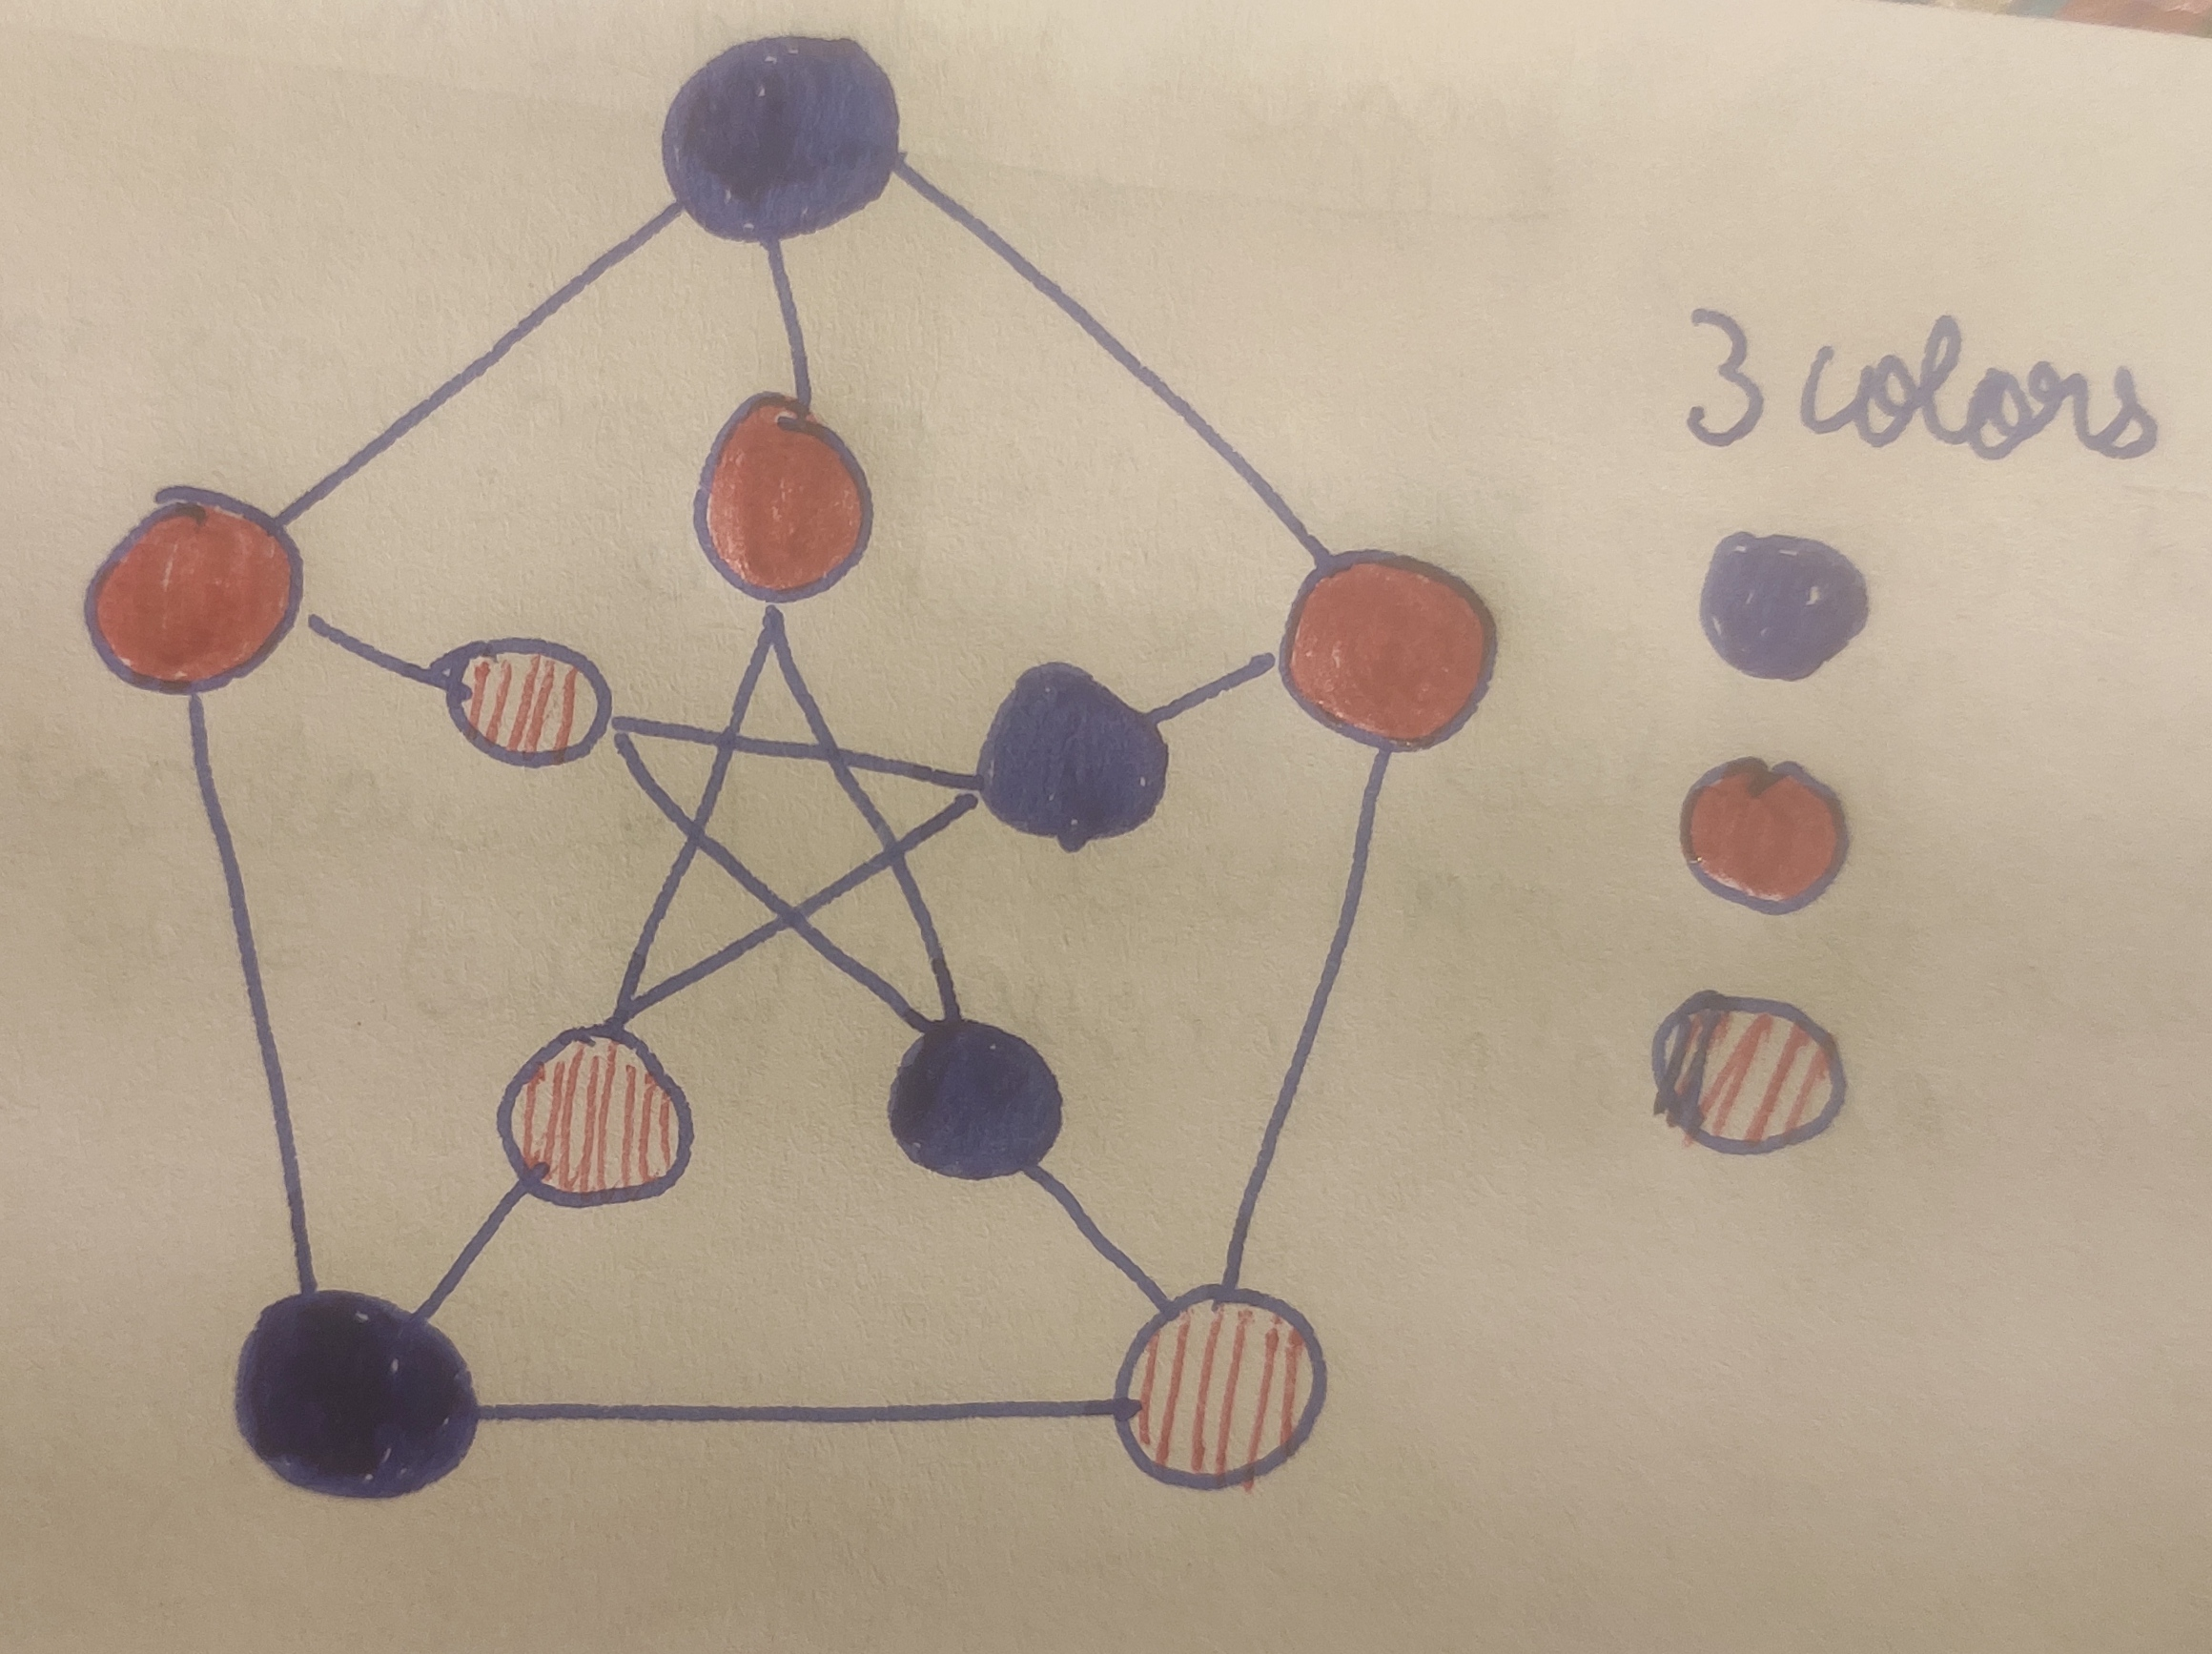
\includegraphics[width=10cm]{q_1.jpg}
    \caption{Found a coloring using 4 colors for G}
    \label{fig:q_1}
\end{figure}

\newpage
\subsection*{Problem 1(2)}
\textit{
    Prove upper bound on $\chi(G)$
}

\solution
Graph $G$ is 3-regular as every vertex has degree 3. And we know for a d-regular graph $\mu_1 = d$. Thus for graph $G$ we have $\mu_1 = 3$, where $\mu_1$ is the largest eigenvalue of the adjacency matrix..

By Wilf's theorem we have $\chi(G) \leq \lfloor \mu_1 \rfloor + 1$ i.e.
\begin{equation}
    \chi(G) \leq 4
\end{equation}

The upper bound we got using Wilf's theorem is larger than the upper bound found found in Problem 1(1). Thus we come to the conclusion
\begin{equation}
    \chi(G) \leq 3
\end{equation}

Now we need to prove 3 is the minimum number of colors needed to color the graph. I am not aware of a theorem that finds a lower bound on $\chi(G)$, so instead I try to prove this by drawing the 1-hop and 2-hop neighborhood of a node and then arguing 3 colors is the minimum number of colors required.

\begin{figure}[H]
    \centering
    \begin{tabular}{cc}
        \subfloat[1-hop neighborhood (2 colors required)]{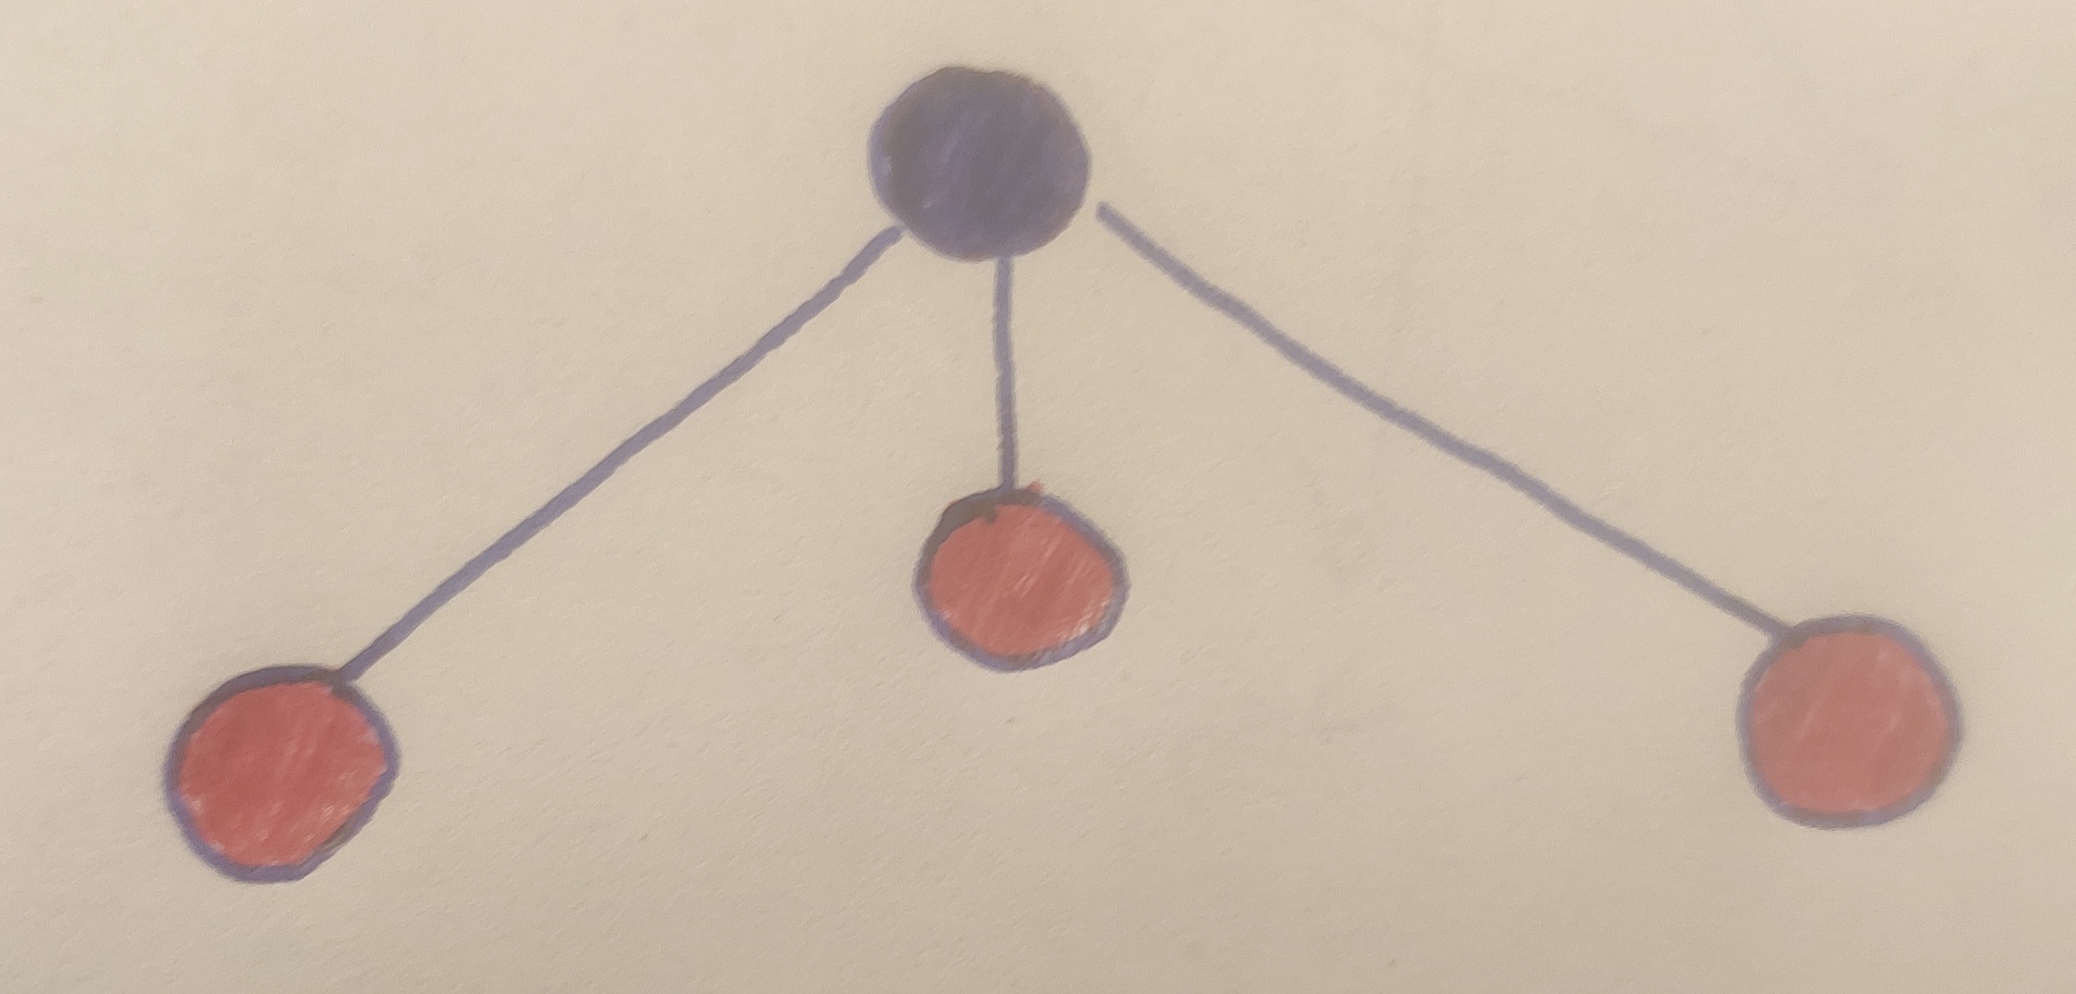
\includegraphics[width=\textwidth/2]{q4_1.jpg}} &
        \subfloat[2-hop neighborhood (dotted line shows existence of edge in original graph)]{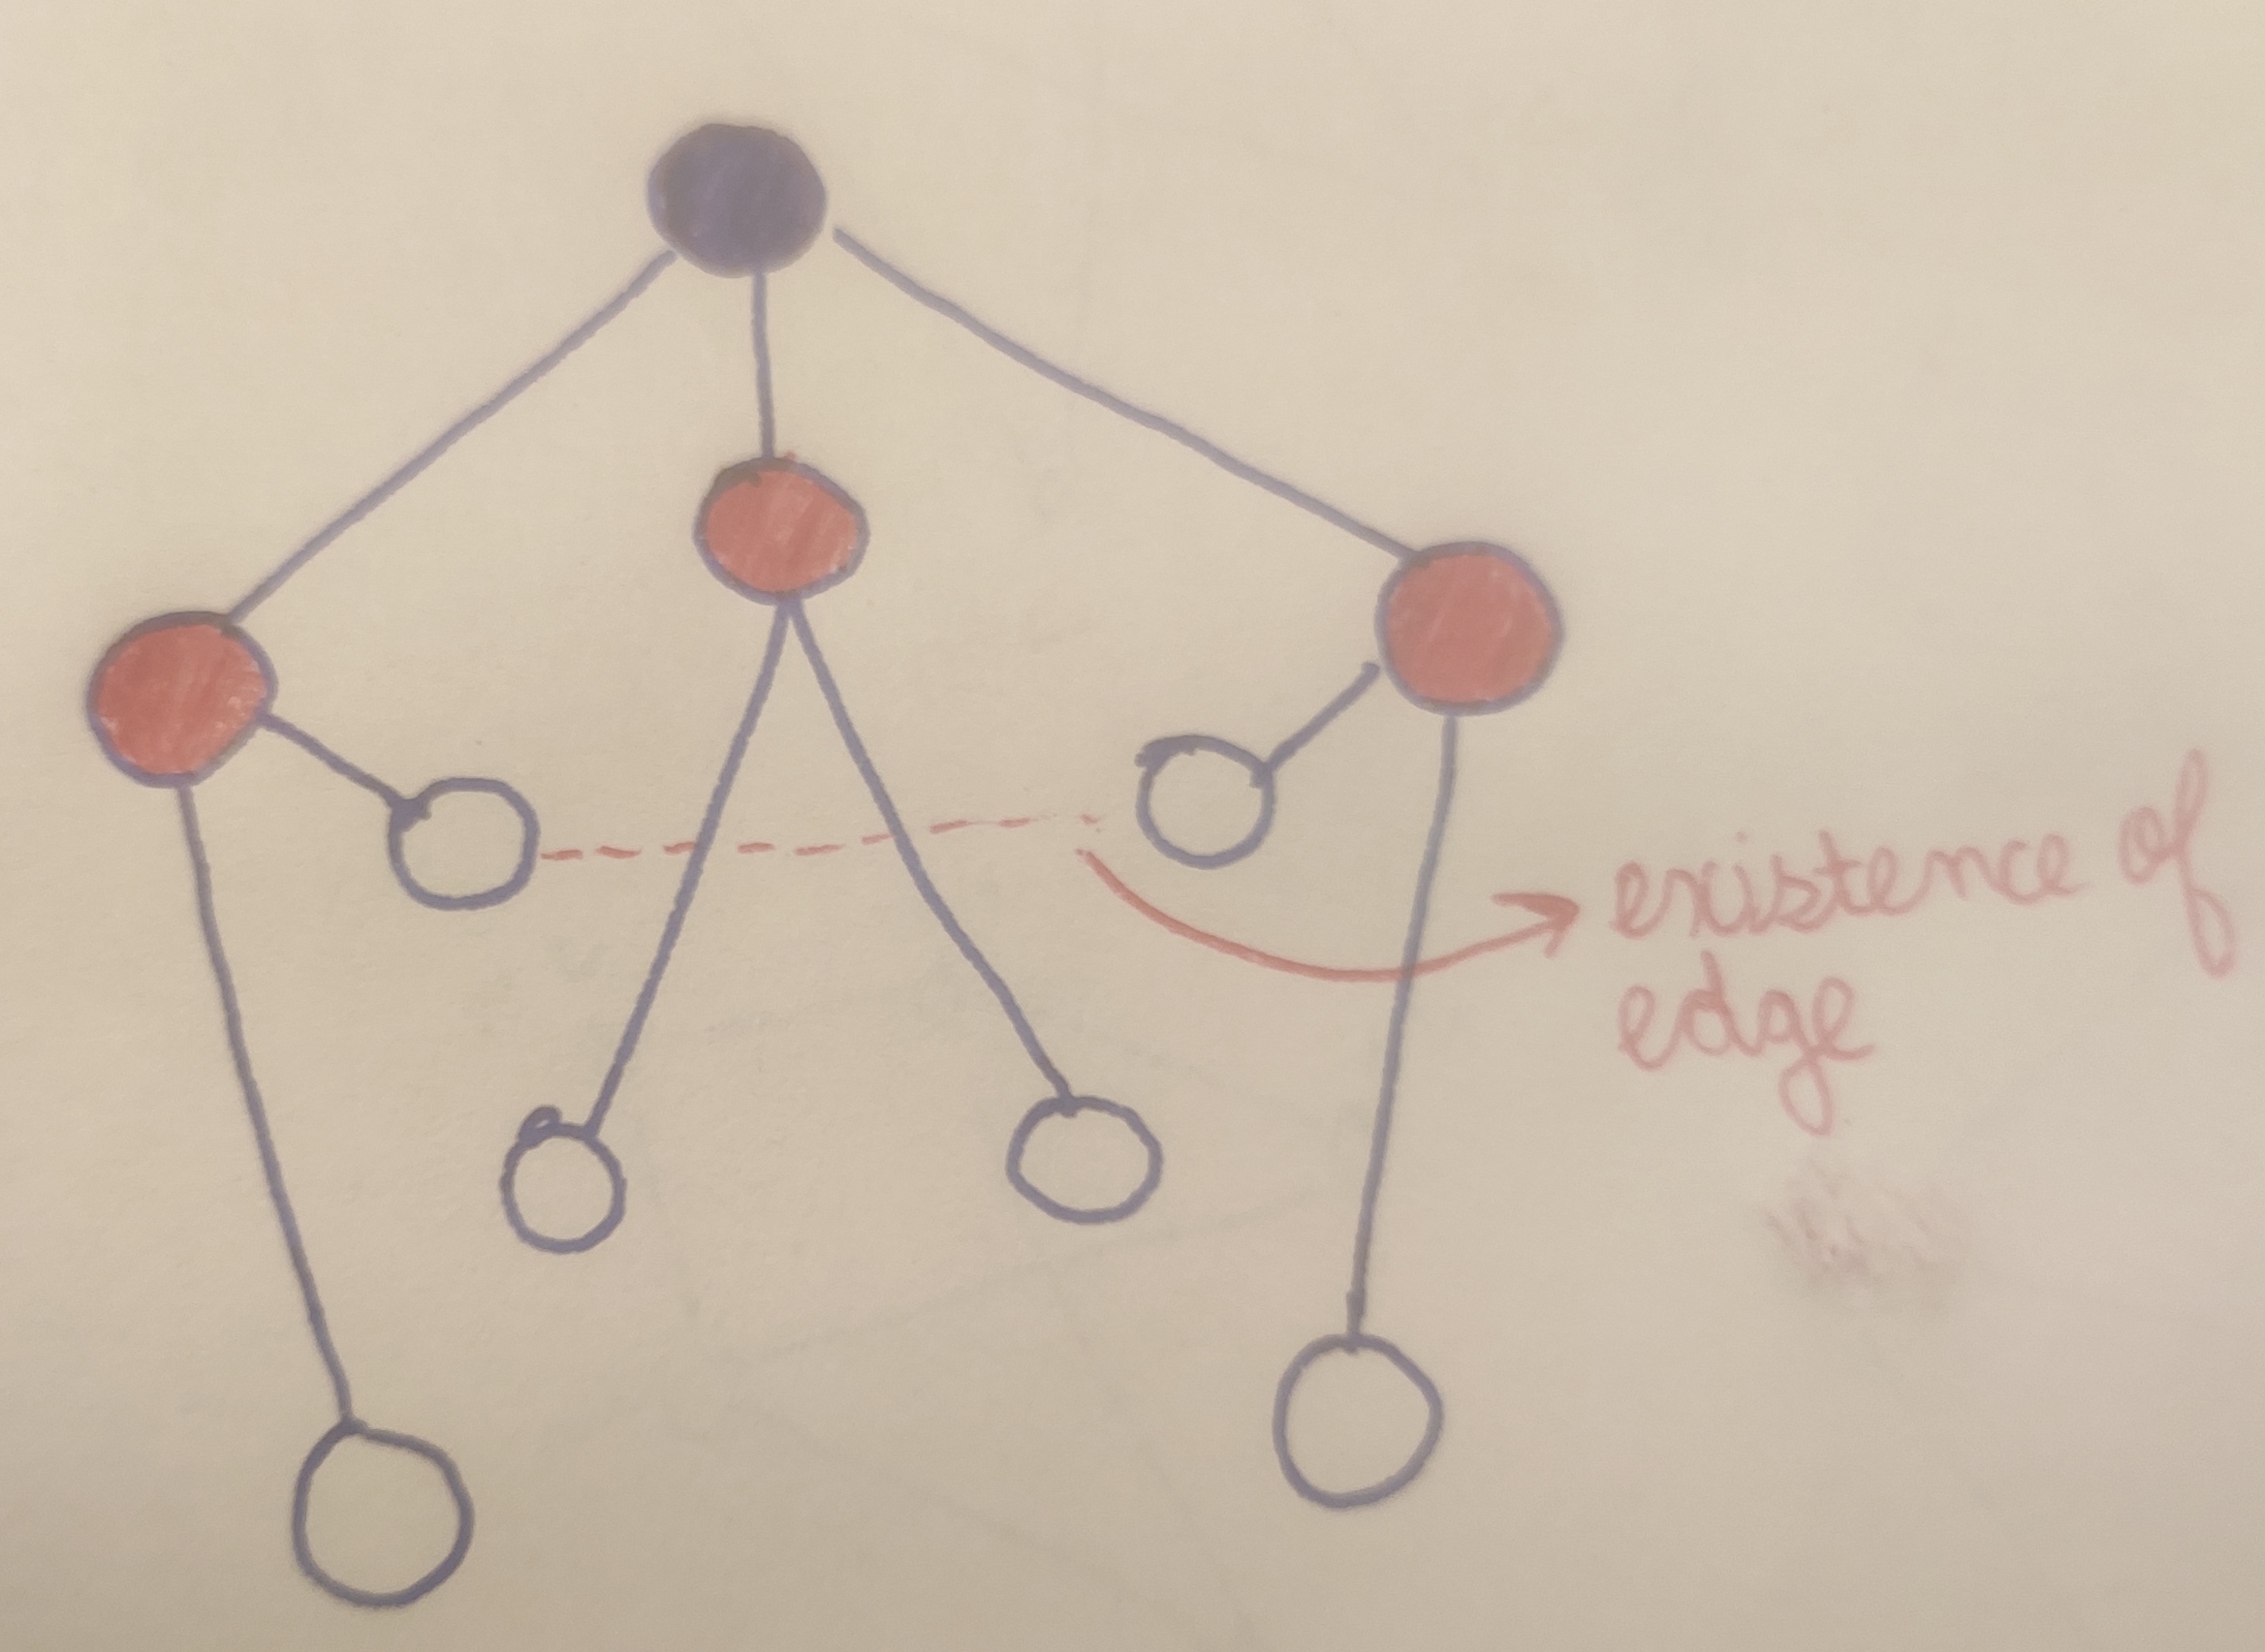
\includegraphics[width=\textwidth/2]{q4_2.jpg}}
    \end{tabular}
    \caption{}
    \label{fig:q_4}
\end{figure}

Figure \ref{fig:q_4} shows why we need minimum of 3 colors to color the graph. We can color all the nodes in 1-hop neighborhood with red color, as they are not connected with each other in original graph. But in case of 2-hop neighborhood, there are some nodes that are connected to the each other in the original graph (like the one shown with dotted line). This means we cannot use blue color for both of these nodes, which means we have to use a third color.

This implies there exists no coloring with fewer than 2 colors.
\rightqed

\newpage
\subsection*{Problem 2}
\textit{
    Find bounds on $\chi(G)$.
}

\solution
Figure \ref{fig:q_2} shows the coloring of the graph with 3 colors, which implies
\begin{equation}
    \chi(G) \leq 3
\end{equation}
\begin{figure}[H]
    \centering
    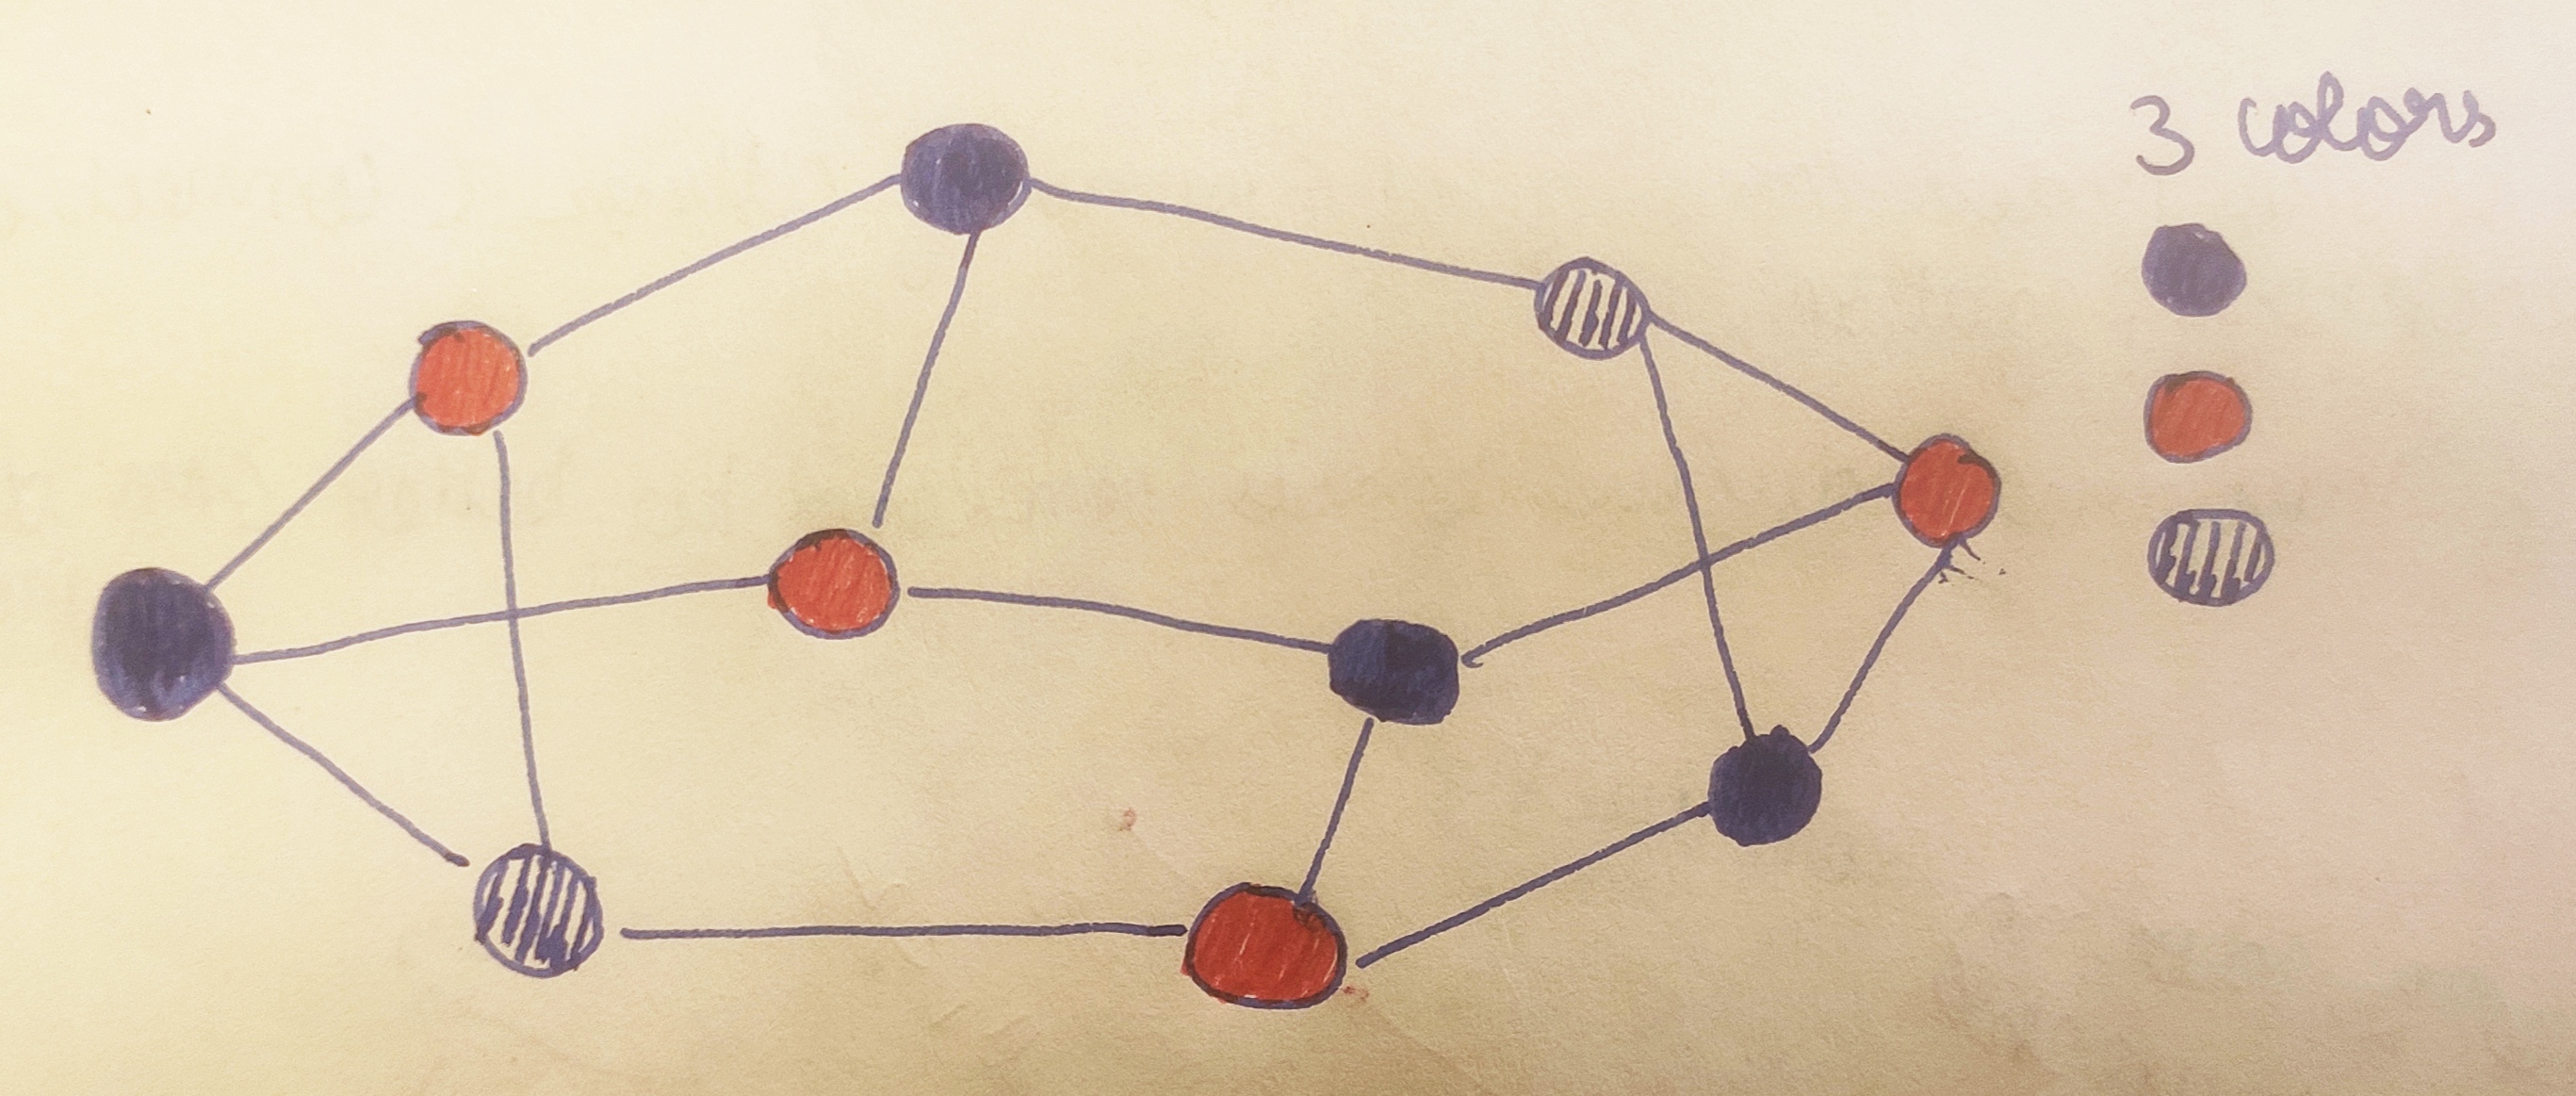
\includegraphics[width=10cm]{q_2.jpg}
    \caption{Found a coloring using 3 colors for G}
    \label{fig:q_2}
\end{figure}

As $G$ is 3-regular graph, we have $\mu_1 = 3$ and by Wilf's theorem $\chi(G) \leq 4$. But we found a more stricter bound which implies
\begin{equation}
    \chi(G) \leq 3
\end{equation}

Not sure of the meaning of the statement "can you compute $\chi(G)$ exactly?". With a similar argument as presented in Problem 1(2), where 1-hop and 2-hop neighborhood were used to prove a lower bound on $\chi(G)$, we can prove that 3 is the minimum number of colors required to color graph $G$.

\newpage
\subsection*{Problem 3}
\textit{
    Find as many eigenvalues as possible.
}

\solution
The original graph can be rearranged to form a bipartite graph as shown in figure \ref{fig:q_3}.
\begin{figure}[H]
    \centering
    \begin{tabular}{cc}
        \subfloat[Providing indexes to each vertex]{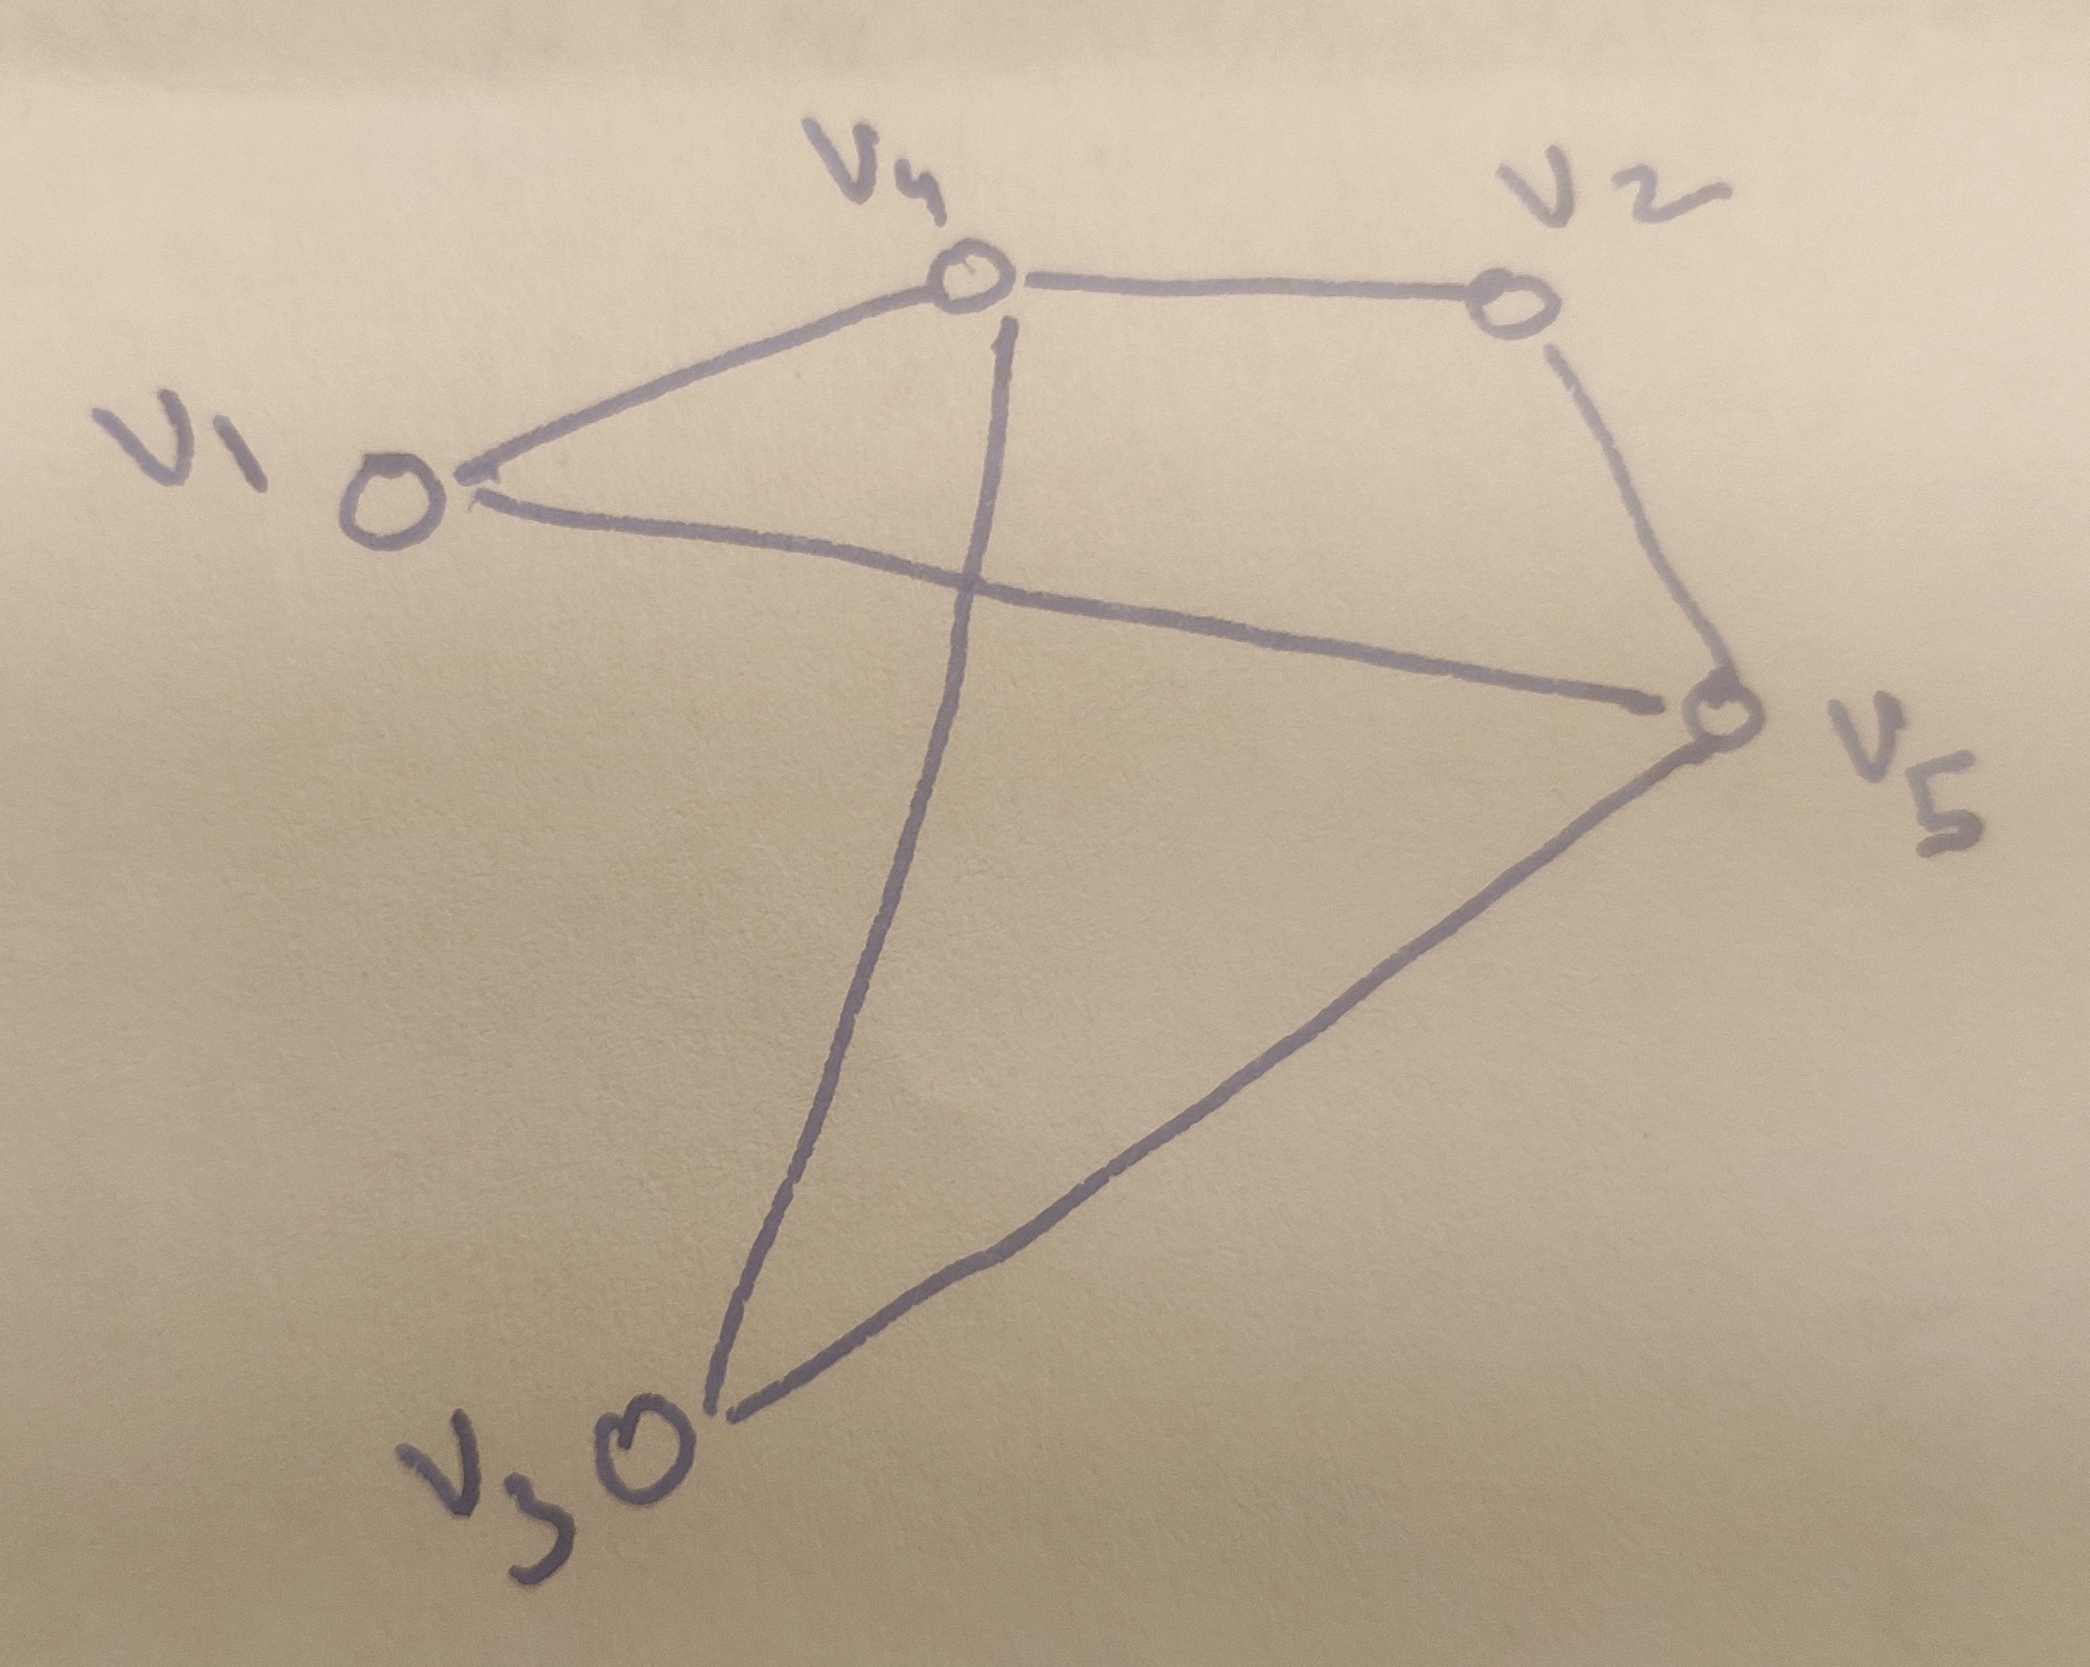
\includegraphics[width=\textwidth/2]{q3_1.jpg}} &
        \subfloat[Rearranging indexes to form a bipartite graph]{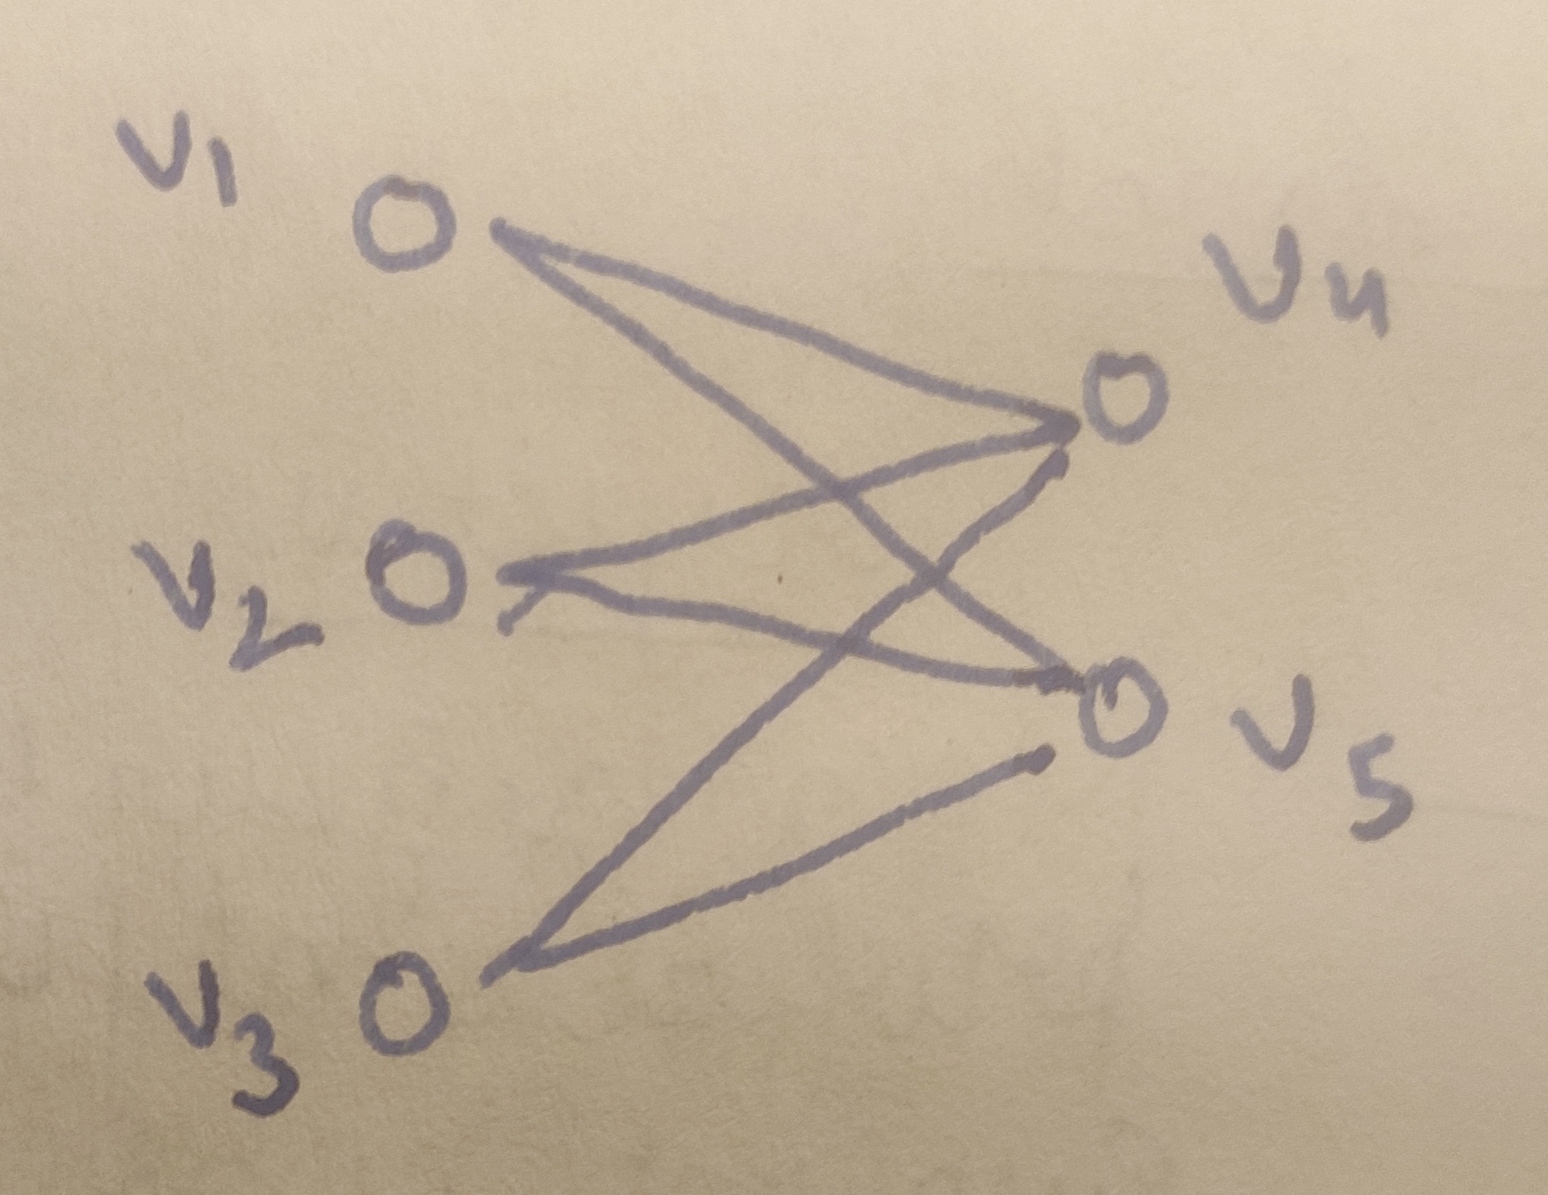
\includegraphics[width=\textwidth/2]{q3_2.jpg}}
    \end{tabular}
    \caption{}
    \label{fig:q_3}
\end{figure}

The adjacency matrix for graph $G$ is given as 
\begin{equation}
    M_G = \begin{bmatrix}
        0 & 0 & 0 & 1 & 1 \\
        0 & 0 & 0 & 1 & 1 \\
        0 & 0 & 0 & 1 & 1 \\
        1 & 1 & 1 & 0 & 0 \\
        1 & 1 & 1 & 0 & 0 \\
    \end{bmatrix}
\end{equation}

We need to find eigenvalues of $M_G$. As $M_G$ is symmetric matrix so we know there must exist 5 real eigenvalues and as proved in class notes we know for a bipartite graph the eigenvalues are symmetric around 0 (this implies 0 is a eigenvalue of $M_G$).

Let the eigenvalues of $M_G$ be $(-\mu_1, -\mu_2, 0, \mu_2, \mu_1)$.

Proving 0 is an eigenvalue. Consider the vector $\vec{x} = [0,0,0,1,-1]^T$, it is trivial to show that $M_G\vec{x} = 0$, which proves $[0,0,0,1,-1]^T$ is a eigenvector with eigenvalue 0 of $M_G$.

Next we use the fact that the eigenvectors of a symmetric matrix are orthogonal to each other. Consider the vector $\vec{y} = [1,-1,0,0,0]^T$. It is orthogonal to $\vec{x}$ i.e. $\langle \vec{x}, \vec{y} \rangle = 0$. By inspection, we find that $M_G\vec{y} = 0$, which implies the eigenvector $\vec{y}$ has eigenvalue 0. As eigenvalues are symmetric around 0, this means $\mu_2 = 0$.

We got 3 three eigenvalues = 0. Now we need to find $\mu_1$.

From the Perron-Frobenius theorem, we know that $\mu_1$ has a strictly positive eigenvector. Let this eigenvector be $\vec{z}$. This vector must also satisfy the conditions $\langle \vec{z}, \vec{x} \rangle = 0$ and $\langle \vec{z}, \vec{y} \rangle = 0$. So suppose $\vec{z} = [a\ b\ c\ d\ e]$. Now by definition we have,
\begin{align*}
    M_G\vec{z} &= \mu_1\vec{z} \\
    \begin{bmatrix}
        0 & 0 & 0 & 1 & 1 \\
        0 & 0 & 0 & 1 & 1 \\
        0 & 0 & 0 & 1 & 1 \\
        1 & 1 & 1 & 0 & 0 \\
        1 & 1 & 1 & 0 & 0 \\
    \end{bmatrix}
    \begin{bmatrix}
        a \\
        b \\
        c \\
        d \\
        e \\
    \end{bmatrix} &= \mu_1
    \begin{bmatrix}
        a \\
        b \\
        c \\
        d \\
        e \\
    \end{bmatrix} \numberthis
\end{align*}

Solving the above equations, we get
\begin{align*}
d + e &= \mu_1a \\
d + e &= \mu_1b \\
d + e &= \mu_1c \\
a + b + c &= \mu_1d \\
a + b + c &= \mu_1e \\
\end{align*}

We know $\mu_1 \neq 0$. Because the adjacency matrix would have atleast one non-zero eigenvalue, which will be used to represent the graph. So from the above equation we get,
\begin{align*}
    a = b = c &= x \text{ (say)} \\
    d = e &= y \text{ (say)}
\end{align*}

Now substituting the above values in $d + e = \mu_1a$ and $a+b+c = \mu_1d$, we get
\begin{align*}
    2y &= \mu_1x \\
    3x &= \mu_1y
\end{align*}

From the above two equations we get the relation between x and y as follows
\begin{equation}
    y = 1.225x
\end{equation}
where $1.225 \approx \sqrt{3/2}$ and we ignore the complex solutions, as we know for symmetric matrix the eigenvectors are real. And solving for $\mu_1$, we get
\begin{equation}
    \mu_1 = \sqrt{6} \approx 2.45
\end{equation}

So we got $\vec{z} = [x\ x\ x\ 1.225x\ 1.225x]^T$. Next we show this is orthogonal to $\vec{x}, \vec{y}$
\begin{align*}
    \langle \vec{z}, \vec{x} \rangle &= 
    \begin{bmatrix}
        x \\ x \\ x \\ 1.225x \\ 1.225x
    \end{bmatrix}^T
    \begin{bmatrix}
        0 \\ 0 \\ 0 \\ 1 \\ -1
    \end{bmatrix}\\
    &= 0 \\
    \langle \vec{z}, \vec{y} \rangle &= 
    \begin{bmatrix}
        x \\ x \\ x \\ 1.225x \\ 1.225x
    \end{bmatrix}^T
    \begin{bmatrix}
        1 \\ -1 \\ 0 \\ 0 \\ 0
    \end{bmatrix}\\
    &= 0
\end{align*}

Now let $x=1$, and we get $\vec{z}=[1\ 1\ 1\ 1.225\ 1.225]$ as the eigenvector of $M_G$ with eigenvalue = 2.45.

The 5 eigenvalues for the adjacency matrix with their corresponding eigenvectors are (from highest to lowest value)
\begin{align}
    2.45 &= \begin{bmatrix}
        1 & 1 & 1 & 1.225 & 1.225
    \end{bmatrix} \\
    0 &= \begin{bmatrix}
        1 & -1 & 0 & 0 & 0
    \end{bmatrix} \\
    0 &= \begin{bmatrix}
        0 & 0 & 0 & 1 & -1
    \end{bmatrix} \\
    0 &= \begin{bmatrix}
        -1 & 1 & 0 & 0 & 0
    \end{bmatrix} \\
    -2.45 &= \begin{bmatrix}
        -1 & -1 & -1 & -1.225 & -1.225
    \end{bmatrix}
\end{align}
\end{document}
